\documentclass[12pt,a4paper]{article}
\usepackage[utf8]{inputenc}
\usepackage{amsmath}
\usepackage{graphicx}
\usepackage{hyperref}
\usepackage{geometry}
\geometry{margin=2.5cm}

\title{Architettura del Computer}
\author{Corso di Sistemi e Reti}

\begin{document}

\maketitle

\section{Introduzione}
L'architettura del computer descrive l'organizzazione e il funzionamento dei componenti di un computer, dalla CPU alla memoria, dai bus ai registri, in modo che possano elaborare informazioni. 

Per un programmatore, comprendere l'architettura del computer è fondamentale per:
\begin{itemize}
    \item Scrivere codice più efficiente e ottimizzato
    \item Capire le prestazioni e i limiti dei programmi
    \item Diagnosticare problemi di performance
    \item Comprendere come il codice ad alto livello viene tradotto in operazioni hardware
\end{itemize}

In questa introduzione vedremo i concetti fondamentali del \textbf{modello di Von Neumann}, della \textbf{CPU}, dell'\textbf{ALU}, dei \textbf{registri}, dei \textbf{bus} e del \textbf{ciclo macchina}.

\section{Modello di Von Neumann}
Il modello di Von Neumann, proposto nel 1945 da John von Neumann, è l'architettura base di quasi tutti i computer moderni. È caratterizzato da:
\begin{itemize}
    \item \textbf{Memoria centrale} unica per dati e istruzioni (stored-program concept).
    \item \textbf{Unità di elaborazione centrale (CPU)} che esegue istruzioni sequenzialmente.
    \item \textbf{Bus di comunicazione} che trasferisce dati e istruzioni tra memoria e CPU.
    \item \textbf{Unità di input/output} per comunicare con l'esterno.
\end{itemize}

\subsection{Il concetto di Stored Program}
Una delle innovazioni più importanti del modello di Von Neumann è che le istruzioni del programma sono memorizzate nella stessa memoria dei dati. Questo significa che:
\begin{itemize}
    \item I programmi possono essere facilmente caricati e modificati
    \item Un programma può modificare se stesso (self-modifying code)
    \item La CPU non distingue tra dati e istruzioni: entrambi sono sequenze di bit
\end{itemize}

\subsection{Il collo di bottiglia di Von Neumann}
Un limite intrinseco di questa architettura è il "Von Neumann bottleneck": CPU e memoria comunicano attraverso un unico bus, limitando la velocità di elaborazione. Le moderne architetture usano cache e parallelismo per mitigare questo problema.

\begin{figure}[h]
    \centering
    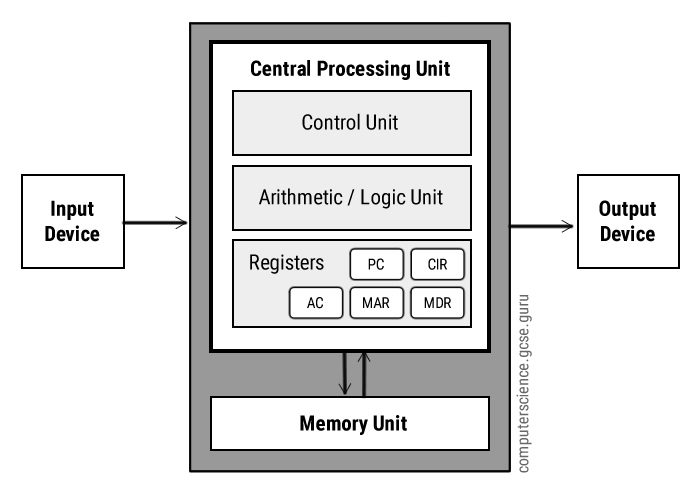
\includegraphics[width=0.6\textwidth]{images/Von-Neumann-Architecture-Diagram.jpg}
    \caption{Schema del modello di Von Neumann}
\end{figure}

\section{CPU (Central Processing Unit)}
La CPU è il cervello del computer e si occupa di:
\begin{itemize}
    \item Prelevare le istruzioni dalla memoria (fetch).
    \item Interpretarle ed eseguirle (decode ed execute).
    \item Gestire il flusso di dati tra memoria e periferiche.
    \item Coordinare tutte le operazioni del sistema.
\end{itemize}

La CPU è composta principalmente da:
\begin{itemize}
    \item \textbf{ALU (Arithmetic Logic Unit)}: esegue operazioni aritmetiche e logiche.
    \item \textbf{Unità di controllo (Control Unit)}: coordina il funzionamento della CPU e del ciclo macchina, genera i segnali di controllo.
    \item \textbf{Registri}: memorie interne velocissime usate per conservare dati temporanei.
    \item \textbf{Cache}: memoria intermedia tra CPU e RAM per accelerare gli accessi.
\end{itemize}

\subsection{Clock e frequenza}
La CPU opera sincronizzata da un clock, un segnale periodico che scandisce le operazioni. La frequenza di clock (misurata in GHz) indica quanti cicli al secondo la CPU può eseguire. Tuttavia, più GHz non significa sempre più prestazioni: conta anche l'architettura e il numero di operazioni per ciclo (IPC - Instructions Per Cycle).

\section{ALU (Arithmetic Logic Unit)}
L'ALU è il componente che esegue tutte le operazioni di calcolo:

\subsection{Operazioni aritmetiche}
\begin{itemize}
    \item Somma, sottrazione
    \item Moltiplicazione, divisione
    \item Operazioni con numeri interi e in virgola mobile (floating point)
\end{itemize}

\subsection{Operazioni logiche}
\begin{itemize}
    \item AND, OR, NOT, XOR (porte logiche)
    \item Shift (spostamento bit a sinistra o destra)
    \item Rotazioni
\end{itemize}

\subsection{Operazioni di confronto}
\begin{itemize}
    \item Maggiore, minore, uguale
    \item Impostazione di flag (Zero, Carry, Overflow, Sign)
\end{itemize}

\textbf{Per il programmatore}: ogni operazione nel codice (come \texttt{a + b}, \texttt{x > y}, \texttt{flag \&\& condition}) viene tradotta in operazioni ALU. Comprendere questo aiuta a capire perché alcune operazioni sono più veloci di altre (es. moltiplicare per 2 con shift vs moltiplicazione).

\section{Registri}
I registri sono memorie ad altissima velocità (tempo di accesso < 1 ns) integrate nella CPU. Sono la memoria più veloce ma anche la più limitata in capacità.

\subsection{Registri principali}
\begin{itemize}
    \item \textbf{Registro accumulatore (ACC)}: memorizza temporaneamente risultati intermedi delle operazioni ALU.
    \item \textbf{Registro istruzioni (IR - Instruction Register)}: contiene l'istruzione corrente da eseguire.
    \item \textbf{Program Counter (PC)}: contiene l'indirizzo della prossima istruzione da eseguire. Viene incrementato automaticamente dopo ogni fetch.
    \item \textbf{Stack Pointer (SP)}: punta alla cima dello stack, usato per chiamate a funzioni e variabili locali.
    \item \textbf{Registri general purpose}: registri usati per memorizzare dati temporanei durante l'esecuzione (es. EAX, EBX, ECX, EDX in architetture x86).
    \item \textbf{Status Register (FLAGS)}: contiene i flag che indicano il risultato delle operazioni (zero, carry, overflow, segno).
\end{itemize}

\subsection{Perché i registri sono importanti per i programmatori}
\begin{itemize}
    \item I compilatori (coloro che traducono il nostro codice in bits) ottimizzano il codice cercando di usare il più possibile i registri invece della RAM
    \item Le variabili locali frequentemente usate vengono mappate in registri
    \item Capire i registri aiuta a leggere codice assembly e debuggare a basso livello
\end{itemize}

\section{Gerarchia di memoria}
La memoria di un computer è organizzata in una gerarchia basata su velocità e capacità:

\begin{enumerate}
    \item \textbf{Registri} (più veloce, ~0.5 ns, ~1 KB)
    \item \textbf{Cache L1} (~1 ns, ~64 KB per core)
    \item \textbf{Cache L2} (~3-10 ns, ~256 KB - 1 MB per core)
    \item \textbf{Cache L3} (~10-20 ns, ~8-32 MB condivisa)
    \item \textbf{RAM} (~50-100 ns, ~4-64 GB)
    \item \textbf{SSD/HDD} (~0.1-10 ms, ~256 GB - 4 TB)
\end{enumerate}

\textbf{Principio di località}: i programmi tendono ad accedere ripetutamente agli stessi dati (località temporale) e a dati vicini in memoria (località spaziale). Le cache sfruttano questo principio per migliorare le prestazioni.

\section{Bus di dati e indirizzi}
I bus sono canali di comunicazione tra i vari componenti del computer. Ogni bus è caratterizzato da una larghezza (numero di bit trasmessi contemporaneamente).

\subsection{Tipi di bus}
\begin{itemize}
    \item \textbf{Bus dati}: trasferisce i dati effettivi tra CPU, memoria e periferiche. La larghezza del bus dati (es. 32 bit, 64 bit) determina quanti dati possono essere trasferiti in un ciclo.
    \item \textbf{Bus indirizzi}: trasporta l'indirizzo di memoria da leggere o scrivere. Un bus indirizzi di $n$ bit può indirizzare $2^n$ locazioni di memoria (es. 32 bit = 4 GB, 64 bit = 16 exabyte teorici).
    \item \textbf{Bus di controllo}: trasmette segnali che coordinano le operazioni (read/write, interrupt, clock, reset).
\end{itemize}

\subsection{Sistemi a 32 bit vs 64 bit}
Un sistema a 64 bit significa che:
\begin{itemize}
    \item I registri sono da 64 bit (possono gestire numeri più grandi)
    \item Il bus indirizzi è da 64 bit (può indirizzare più di 4 GB di RAM)
    \item Le istruzioni operano su parole da 64 bit
\end{itemize}

\section{Ciclo macchina (Fetch-Decode-Execute)}
Il ciclo macchina descrive il processo attraverso cui la CPU esegue le istruzioni. È un ciclo continuo e ripetitivo:

\begin{enumerate}
    \item \textbf{Fetch (prelievo)}: 
    \begin{itemize}
        \item La CPU legge l'istruzione dalla memoria all'indirizzo indicato dal PC
        \item L'istruzione viene caricata nel registro IR
        \item Il PC viene incrementato per puntare alla prossima istruzione
    \end{itemize}
    
    \item \textbf{Decode (decodifica)}: 
    \begin{itemize}
        \item L'unità di controllo interpreta l'istruzione
        \item Identifica l'operazione da compiere e gli operandi necessari
        \item Prepara i segnali di controllo per l'ALU e altri componenti
    \end{itemize}
    
    \item \textbf{Execute (esecuzione)}: 
    \begin{itemize}
        \item L'ALU esegue l'operazione richiesta (calcolo, confronto, ecc.)
        \item Vengono letti i dati dai registri o dalla memoria
        \item Vengono aggiornati i flag di stato
    \end{itemize}
    
    \item \textbf{Store (memorizzazione)}: 
    \begin{itemize}
        \item Il risultato viene scritto in un registro o nella memoria
        \item Lo stato della CPU viene aggiornato
    \end{itemize}
\end{enumerate}

\subsection{Esempio pratico}
Consideriamo l'istruzione: \texttt{ADD R1, R2, R3} (R1 = R2 + R3)

\begin{enumerate}
    \item \textbf{Fetch}: preleva l'istruzione dalla memoria
    \item \textbf{Decode}: riconosce ADD e identifica i registri R1, R2, R3
    \item \textbf{Execute}: l'ALU somma i valori di R2 e R3
    \item \textbf{Store}: il risultato viene scritto in R1
\end{enumerate}

\subsection{Pipeline e parallelismo}
Le CPU moderne usano la pipeline per eseguire più istruzioni contemporaneamente in fasi diverse:
\begin{itemize}
    \item Mentre un'istruzione è in Execute, la successiva è in Decode e un'altra in Fetch
    \item Questo aumenta il throughput (istruzioni al secondo)
    \item Complicazioni: hazard, branch prediction, out-of-order execution
\end{itemize}

\section{Linguaggi di programmazione e hardware}
\subsection{Livelli di astrazione}
\begin{enumerate}
    \item \textbf{Linguaggio macchina}: codice binario eseguito direttamente dalla CPU
    \item \textbf{Assembly}: rappresentazione simbolica del linguaggio macchina
    \item \textbf{Linguaggi di basso livello}: C, C++ (controllo diretto su memoria e hardware)
    \item \textbf{Linguaggi di alto livello}: Python, Java, JavaScript (forte astrazione dall'hardware)
\end{enumerate}

\subsection{Compilazione vs Interpretazione}
\begin{itemize}
    \item \textbf{Linguaggi compilati} (C, C++, Rust): tradotti completamente in codice macchina prima dell'esecuzione. Più veloci ma meno portabili.
    \item \textbf{Linguaggi interpretati} (Python, JavaScript): eseguiti riga per riga da un interprete. Più lenti ma più flessibili.
    \item \textbf{Linguaggi intermedi} (Java, C\#): compilati in bytecode ed eseguiti da una macchina virtuale (JVM, CLR).
\end{itemize}

\section{Concetti essenziali per programmatori}

\subsection{Rappresentazione dei dati}
\begin{itemize}
    \item \textbf{Bit e byte}: tutte le informazioni sono rappresentate in binario
    \item \textbf{Tipi di dati}: int (32 bit), long (64 bit), float (32 bit), double (64 bit)
    \item \textbf{Endianness}: ordine dei byte (big-endian vs little-endian)
    \item \textbf{Overflow}: cosa succede quando un calcolo supera la capacità del tipo
\end{itemize}

\subsection{Memoria: unità di misura e conversioni}

\subsubsection{Unità di misura}
La memoria del computer si misura in potenze di 2. Le unità principali sono:

\begin{itemize}
    \item \textbf{Bit (b)}: l'unità elementare, può valere 0 o 1
    \item \textbf{Byte (B)}: 8 bit = 1 Byte
    \item \textbf{Kilobyte (KB)}: $2^{10}$ Byte = 1.024 Byte $\approx$ 1.000 Byte
    \item \textbf{Megabyte (MB)}: $2^{20}$ Byte = 1.048.576 Byte $\approx$ 1.000.000 Byte
    \item \textbf{Gigabyte (GB)}: $2^{30}$ Byte = 1.073.741.824 Byte $\approx$ 1.000.000.000 Byte
    \item \textbf{Terabyte (TB)}: $2^{40}$ Byte = 1.099.511.627.776 Byte $\approx$ 1.000.000.000.000 Byte
\end{itemize}

\textbf{Nota importante}: esiste una differenza tra unità binarie (KB, MB, GB) e unità decimali (kB, MB, GB secondo lo standard SI). Nelle specifiche dei produttori di storage si usano spesso le unità decimali (1 GB = $10^9$ byte), mentre i sistemi operativi usano quelle binarie.

\subsubsection{Formule di conversione}
\begin{itemize}
    \item Da bit a Byte: dividere per 8
    \item Da Byte a bit: moltiplicare per 8
    \item Da KB a Byte: moltiplicare per 1.024
    \item Da MB a KB: moltiplicare per 1.024
    \item Da GB a MB: moltiplicare per 1.024
    \item In generale: per salire di livello moltiplicare per 1.024, per scendere dividere per 1.024
\end{itemize}

\subsubsection{Esercizi svolti}

\textbf{Esercizio 1}: Converti 4096 bit in Byte.

\textbf{Soluzione}:
\[
4096 \text{ bit} \div 8 = 512 \text{ Byte}
\]

\textbf{Esercizio 2}: Converti 2 GB in MB.

\textbf{Soluzione}:
\[
2 \text{ GB} \times 1.024 = 2.048 \text{ MB}
\]

\textbf{Esercizio 3}: Converti 500 MB in bit.

\textbf{Soluzione}:
\begin{align*}
500 \text{ MB} &= 500 \times 1.024 \text{ KB} = 512.000 \text{ KB} \\
&= 512.000 \times 1.024 \text{ Byte} = 524.288.000 \text{ Byte} \\
&= 524.288.000 \times 8 \text{ bit} = 4.194.304.000 \text{ bit}
\end{align*}

\textbf{Esercizio 4}: Un file occupa 8.388.608 bit. Quanti MB sono?

\textbf{Soluzione}:
\begin{align*}
8.388.608 \text{ bit} &\div 8 = 1.048.576 \text{ Byte} \\
&\div 1.024 = 1.024 \text{ KB} \\
&\div 1.024 = 1 \text{ MB}
\end{align*}

\textbf{Esercizio 5}: Una memoria RAM è da 16 GB. Quanti byte può contenere?

\textbf{Soluzione}:
\[
16 \text{ GB} = 16 \times 1.024^3 \text{ Byte} = 16 \times 1.073.741.824 = 17.179.869.184 \text{ Byte}
\]

\subsubsection{Esercizi da svolgere}

\textbf{Esercizio 1}: Converti 2048 Byte in KB.

\textbf{Esercizio 2}: Converti 5 GB in Byte.

\textbf{Esercizio 3}: Un video occupa 750 MB. Quanti bit sono?

\textbf{Esercizio 4}: Una chiavetta USB ha capacità di 32 GB. Quanti file da 4 MB ciascuno può contenere?

\textbf{Esercizio 5}: Un disco rigido da 2 TB quanti GB contiene? E quanti MB?

\subsubsection{Soluzioni degli esercizi}

\textbf{Soluzione Esercizio 1}: 
\[
2048 \text{ Byte} \div 1.024 = 2 \text{ KB}
\]

\textbf{Soluzione Esercizio 2}:
\[
5 \text{ GB} = 5 \times 1.024^3 = 5.368.709.120 \text{ Byte}
\]

\textbf{Soluzione Esercizio 3}:
\begin{align*}
750 \text{ MB} &= 750 \times 1.024 \times 1.024 \text{ Byte} = 786.432.000 \text{ Byte} \\
&= 786.432.000 \times 8 = 6.291.456.000 \text{ bit}
\end{align*}

\textbf{Soluzione Esercizio 4}:
\begin{align*}
32 \text{ GB} &= 32 \times 1.024 \text{ MB} = 32.768 \text{ MB} \\
32.768 \text{ MB} &\div 4 \text{ MB} = 8.192 \text{ file}
\end{align*}

\textbf{Soluzione Esercizio 5}:
\begin{align*}
2 \text{ TB} &= 2 \times 1.024 \text{ GB} = 2.048 \text{ GB} \\
2.048 \text{ GB} &= 2.048 \times 1.024 \text{ MB} = 2.097.152 \text{ MB}
\end{align*}

\subsection{Puntatori e indirizzi di memoria}
\begin{itemize}
    \item Un puntatore contiene l'indirizzo di memoria di un dato
    \item Fondamentali in C/C++ per gestire memoria dinamica
    \item Permettono di passare parametri per riferimento
    \item Errori comuni: segmentation fault, memory leak, dangling pointer
\end{itemize}

\subsection{Stack e Heap}
\begin{itemize}
    \item \textbf{Stack}: memoria automatica per variabili locali e chiamate a funzione. LIFO (Last In First Out). Veloce ma limitata.
    \item \textbf{Heap}: memoria dinamica allocata con malloc/new. Più lenta ma flessibile. Va gestita manualmente (free/delete).
\end{itemize}

\subsection{Performance e ottimizzazione}
\begin{itemize}
    \item \textbf{Cache-friendly code}: accedere ai dati in modo sequenziale sfrutta la cache
    \item \textbf{Branch prediction}: evitare if complessi in loop critici
    \item \textbf{Allineamento dati}: struct e array allineati sono più veloci
    \item \textbf{SIMD}: Single Instruction Multiple Data per parallelismo
\end{itemize}

\section{Conclusione}
Questi concetti costituiscono la base per comprendere come funziona un computer. Per un programmatore, capire l'architettura hardware significa:

\begin{itemize}
    \item Scrivere codice più efficiente
    \item Comprendere i limiti e le possibilità dell'hardware
    \item Debuggare problemi complessi
    \item Fare scelte architetturali migliori nei propri progetti
\end{itemize}

Il modello di Von Neumann, il ruolo della CPU e dei registri, l'importanza dei bus e il ciclo macchina sono alla base di ogni sistema di calcolo moderno. Anche se i linguaggi di alto livello astraggono molto dall'hardware, conoscere questi fondamenti distingue un buon programmatore da uno eccellente.

\end{document}
